\documentclass[letterpaper,12pt]{article}
\usepackage[margin=.5in]{geometry}
\usepackage{tikz}
\usepackage{helvet}
\renewcommand{\familydefault}{\sfdefault}
\pagestyle{empty}
\pdfmapfile{+cm.map}
\pdfmapfile{+ps2pk35.map}
\setlength{\parindent}{0pt}
\hyphenpenalty=10000
\exhyphenpenalty=10000
\begin{document}
\null\begin{tikzpicture}[remember picture,overlay,x=1cm,y=1cm]
\begin{scope}[shift={(current page.north west)}]
\node[anchor=north west,inner sep=0pt,font=\fontsize{11.5}{13}\selectfont] at (1.4,-.72) {Week 33 / Prime-length necklaces / Grades 2--3};
\node[anchor=south west,inner sep=0pt,font=\fontsize{9}{11}\selectfont] at (1.4,-27.2) {Bellingham Math Circle / Week 33 / F33-23-v5};
\node[anchor=south east,inner sep=0pt,font=\fontsize{9}{11}\selectfont] at (20.15,-27.2) {1};
\begin{scope}[shift={(1.4,-1.65)}]
\node[anchor=north west,inner sep=0pt,align=left,text width=18.5cm,font=\fontsize{13}{16.38}\selectfont] at (0,0) {Each bead may be A or B; one-color rings are allowed. Read clockwise from the start arrow. The bead order is the readout. Rings count as the same when turning makes them match. Keep them face up; do not flip them over.};
\draw[gray!65,line width=.7pt] (2.5,-4.6) circle (1.3cm);
\draw[fill=white] (2.5000,-3.3000) circle (0.29cm);
\node[font=\fontsize{12}{14}\selectfont,inner sep=1pt] at (2.5,-3.3) {A};
\draw[fill=white] (3.6258,-5.2500) circle (0.29cm);
\node[font=\fontsize{12}{14}\selectfont,inner sep=1pt] at (3.6258330249197703,-5.249999999999999) {A};
\draw[fill=gray!65] (1.3742,-5.2500) circle (0.29cm);
\node[font=\fontsize{12}{14}\selectfont,inner sep=1pt] at (1.37416697508023,-5.25) {B};
\draw[->,line width=.8pt] (2.5,-2.3499999999999996) -- (2.5,-2.8899999999999997);
\node[font=\fontsize{9}{11}\selectfont,inner sep=1pt] at (2.5,-2.1499999999999995) {start};
\draw[->,line width=.7pt] (0.9498,-3.7050) arc[start angle=150,end angle=110,radius=1.79cm];
\node[font=\fontsize{15}{17}\selectfont,inner sep=1pt] at (2.5,-6.65) {AAB};
\draw[gray!65,line width=.7pt] (8.5,-4.6) circle (1.3cm);
\draw[fill=white] (8.5000,-3.3000) circle (0.29cm);
\node[font=\fontsize{12}{14}\selectfont,inner sep=1pt] at (8.5,-3.3) {A};
\draw[fill=white] (9.6258,-5.2500) circle (0.29cm);
\node[font=\fontsize{12}{14}\selectfont,inner sep=1pt] at (9.625833024919771,-5.249999999999999) {A};
\draw[fill=gray!65] (7.3742,-5.2500) circle (0.29cm);
\node[font=\fontsize{12}{14}\selectfont,inner sep=1pt] at (7.37416697508023,-5.25) {B};
\draw[->,line width=.8pt] (10.448557158514987,-5.725) -- (9.98090344047139,-5.454999999999999);
\node[font=\fontsize{9}{11}\selectfont,inner sep=1pt] at (9.625833024919771,-5.8999999999999995) {start};
\draw[->,line width=.7pt] (6.9498,-3.7050) arc[start angle=150,end angle=110,radius=1.79cm];
\node[font=\fontsize{15}{17}\selectfont,inner sep=1pt] at (8.5,-6.65) {ABA};
\draw[gray!65,line width=.7pt] (14.5,-4.6) circle (1.3cm);
\draw[fill=white] (14.5000,-3.3000) circle (0.29cm);
\node[font=\fontsize{12}{14}\selectfont,inner sep=1pt] at (14.5,-3.3) {A};
\draw[fill=white] (15.6258,-5.2500) circle (0.29cm);
\node[font=\fontsize{12}{14}\selectfont,inner sep=1pt] at (15.625833024919771,-5.249999999999999) {A};
\draw[fill=gray!65] (13.3742,-5.2500) circle (0.29cm);
\node[font=\fontsize{12}{14}\selectfont,inner sep=1pt] at (13.37416697508023,-5.25) {B};
\draw[->,line width=.8pt] (12.551442841485013,-5.7250000000000005) -- (13.01909655952861,-5.455);
\node[font=\fontsize{9}{11}\selectfont,inner sep=1pt] at (13.37416697508023,-5.9) {start};
\draw[->,line width=.7pt] (12.9498,-3.7050) arc[start angle=150,end angle=110,radius=1.79cm];
\node[font=\fontsize{15}{17}\selectfont,inner sep=1pt] at (14.5,-6.65) {BAA};
\draw[->,line width=.8pt] (4.4,-4.6) -- (6.45,-4.6);
\draw[->,line width=.8pt] (10.4,-4.6) -- (12.45,-4.6);
\node[anchor=north west,inner sep=0pt,align=left,text width=3cm,font=\fontsize{10}{12.6}\selectfont] at (4.4,-3.1) {move start};
\node[anchor=north west,inner sep=0pt,align=left,text width=3cm,font=\fontsize{10}{12.6}\selectfont] at (10.4,-3.1) {move start};
\node[anchor=north west,inner sep=0pt,align=left,text width=18.6cm,font=\fontsize{14}{17.78}\selectfont] at (0,-7.8) {\textbf{Problem 1:} Make every different three-bead ring using A and B. Find all its readouts as you move the start.};
\draw[gray!65,line width=.7pt] (2.7,-12.35) circle (1.75cm);
\draw[fill=white] (2.7000,-10.6000) circle (0.42cm);
\draw[fill=white] (4.2155,-13.2250) circle (0.42cm);
\draw[fill=white] (1.1845,-13.2250) circle (0.42cm);
\draw[->,line width=.7pt] (0.6475,-11.1650) arc[start angle=150,end angle=110,radius=2.37cm];
\draw[gray!45,line width=.35pt] (5.3,-11.2) -- (9.0,-11.2);
\draw[gray!45,line width=.35pt] (5.3,-12.35) -- (9.0,-12.35);
\draw[gray!45,line width=.35pt] (5.3,-13.5) -- (9.0,-13.5);
\draw[gray!65,line width=.7pt] (12.0,-12.35) circle (1.75cm);
\draw[fill=white] (12.0000,-10.6000) circle (0.42cm);
\draw[fill=white] (13.5155,-13.2250) circle (0.42cm);
\draw[fill=white] (10.4845,-13.2250) circle (0.42cm);
\draw[->,line width=.7pt] (9.9475,-11.1650) arc[start angle=150,end angle=110,radius=2.37cm];
\draw[gray!45,line width=.35pt] (14.6,-11.2) -- (18.5,-11.2);
\draw[gray!45,line width=.35pt] (14.6,-12.35) -- (18.5,-12.35);
\draw[gray!45,line width=.35pt] (14.6,-13.5) -- (18.5,-13.5);
\draw[gray!65,line width=.7pt] (2.7,-17.45) circle (1.75cm);
\draw[fill=white] (2.7000,-15.7000) circle (0.42cm);
\draw[fill=white] (4.2155,-18.3250) circle (0.42cm);
\draw[fill=white] (1.1845,-18.3250) circle (0.42cm);
\draw[->,line width=.7pt] (0.6475,-16.2650) arc[start angle=150,end angle=110,radius=2.37cm];
\draw[gray!45,line width=.35pt] (5.3,-16.3) -- (9.0,-16.3);
\draw[gray!45,line width=.35pt] (5.3,-17.45) -- (9.0,-17.45);
\draw[gray!45,line width=.35pt] (5.3,-18.6) -- (9.0,-18.6);
\draw[gray!65,line width=.7pt] (12.0,-17.45) circle (1.75cm);
\draw[fill=white] (12.0000,-15.7000) circle (0.42cm);
\draw[fill=white] (13.5155,-18.3250) circle (0.42cm);
\draw[fill=white] (10.4845,-18.3250) circle (0.42cm);
\draw[->,line width=.7pt] (9.9475,-16.2650) arc[start angle=150,end angle=110,radius=2.37cm];
\draw[gray!45,line width=.35pt] (14.6,-16.3) -- (18.5,-16.3);
\draw[gray!45,line width=.35pt] (14.6,-17.45) -- (18.5,-17.45);
\draw[gray!45,line width=.35pt] (14.6,-18.6) -- (18.5,-18.6);
\draw[gray!65,line width=.7pt] (2.7,-22.549999999999997) circle (1.75cm);
\draw[fill=white] (2.7000,-20.8000) circle (0.42cm);
\draw[fill=white] (4.2155,-23.4250) circle (0.42cm);
\draw[fill=white] (1.1845,-23.4250) circle (0.42cm);
\draw[->,line width=.7pt] (0.6475,-21.3650) arc[start angle=150,end angle=110,radius=2.37cm];
\draw[gray!45,line width=.35pt] (5.3,-21.4) -- (9.0,-21.4);
\draw[gray!45,line width=.35pt] (5.3,-22.549999999999997) -- (9.0,-22.549999999999997);
\draw[gray!45,line width=.35pt] (5.3,-23.7) -- (9.0,-23.7);
\draw[gray!65,line width=.7pt] (12.0,-22.549999999999997) circle (1.75cm);
\draw[fill=white] (12.0000,-20.8000) circle (0.42cm);
\draw[fill=white] (13.5155,-23.4250) circle (0.42cm);
\draw[fill=white] (10.4845,-23.4250) circle (0.42cm);
\draw[->,line width=.7pt] (9.9475,-21.3650) arc[start angle=150,end angle=110,radius=2.37cm];
\draw[gray!45,line width=.35pt] (14.6,-21.4) -- (18.5,-21.4);
\draw[gray!45,line width=.35pt] (14.6,-22.549999999999997) -- (18.5,-22.549999999999997);
\draw[gray!45,line width=.35pt] (14.6,-23.7) -- (18.5,-23.7);\end{scope}\end{scope}\end{tikzpicture}
\newpage
\null\begin{tikzpicture}[remember picture,overlay,x=1cm,y=1cm]
\begin{scope}[shift={(current page.north west)}]
\node[anchor=north west,inner sep=0pt,font=\fontsize{11.5}{13}\selectfont] at (1.4,-.72) {Week 33 / Prime-length necklaces / Grades 2--3};
\node[anchor=south west,inner sep=0pt,font=\fontsize{9}{11}\selectfont] at (1.4,-27.2) {Bellingham Math Circle / Week 33 / F33-23-v5};
\node[anchor=south east,inner sep=0pt,font=\fontsize{9}{11}\selectfont] at (20.15,-27.2) {2};
\begin{scope}[shift={(1.4,-1.65)}]
\node[anchor=north west,inner sep=0pt,align=left,text width=18.6cm,font=\fontsize{14}{17.78}\selectfont] at (0,0) {\textbf{Problem 2:} Group cards that make the same ring. How many groups are there, and how many cards are in each group?};
\draw[line width=.65pt] (0.0,-2.5) rectangle (8.8,-6.4);
\draw[fill=white] (2.9000000000000004,-4.2) circle (0.47cm);
\node[font=\fontsize{15}{17}\selectfont,inner sep=1pt] at (2.9000000000000004,-4.2) {A};
\draw[fill=white] (4.4,-4.2) circle (0.47cm);
\node[font=\fontsize{15}{17}\selectfont,inner sep=1pt] at (4.4,-4.2) {A};
\draw[fill=white] (5.9,-4.2) circle (0.47cm);
\node[font=\fontsize{15}{17}\selectfont,inner sep=1pt] at (5.9,-4.2) {A};
\node[font=\fontsize{10}{12}\selectfont,inner sep=1pt] at (2.9000000000000004,-2.8) {start};
\draw[->,line width=.6pt] (2.4300000000000006,-5.95) -- (6.37,-5.95);
\node[font=\fontsize{9}{11}\selectfont,inner sep=1pt] at (8.55,-2.8) {1};
\draw[line width=.65pt] (9.5,-2.5) rectangle (18.3,-6.4);
\draw[fill=white] (12.4,-4.2) circle (0.47cm);
\node[font=\fontsize{15}{17}\selectfont,inner sep=1pt] at (12.4,-4.2) {A};
\draw[fill=white] (13.9,-4.2) circle (0.47cm);
\node[font=\fontsize{15}{17}\selectfont,inner sep=1pt] at (13.9,-4.2) {A};
\draw[fill=gray!60] (15.4,-4.2) circle (0.47cm);
\node[font=\fontsize{15}{17}\selectfont,inner sep=1pt] at (15.4,-4.2) {B};
\node[font=\fontsize{10}{12}\selectfont,inner sep=1pt] at (12.4,-2.8) {start};
\draw[->,line width=.6pt] (11.93,-5.95) -- (15.870000000000001,-5.95);
\node[font=\fontsize{9}{11}\selectfont,inner sep=1pt] at (18.05,-2.8) {2};
\draw[line width=.65pt] (0.0,-7.6) rectangle (8.8,-11.5);
\draw[fill=white] (2.9000000000000004,-9.299999999999999) circle (0.47cm);
\node[font=\fontsize{15}{17}\selectfont,inner sep=1pt] at (2.9000000000000004,-9.299999999999999) {A};
\draw[fill=gray!60] (4.4,-9.299999999999999) circle (0.47cm);
\node[font=\fontsize{15}{17}\selectfont,inner sep=1pt] at (4.4,-9.299999999999999) {B};
\draw[fill=white] (5.9,-9.299999999999999) circle (0.47cm);
\node[font=\fontsize{15}{17}\selectfont,inner sep=1pt] at (5.9,-9.299999999999999) {A};
\node[font=\fontsize{10}{12}\selectfont,inner sep=1pt] at (2.9000000000000004,-7.8999999999999995) {start};
\draw[->,line width=.6pt] (2.4300000000000006,-11.05) -- (6.37,-11.05);
\node[font=\fontsize{9}{11}\selectfont,inner sep=1pt] at (8.55,-7.8999999999999995) {3};
\draw[line width=.65pt] (9.5,-7.6) rectangle (18.3,-11.5);
\draw[fill=white] (12.4,-9.299999999999999) circle (0.47cm);
\node[font=\fontsize{15}{17}\selectfont,inner sep=1pt] at (12.4,-9.299999999999999) {A};
\draw[fill=gray!60] (13.9,-9.299999999999999) circle (0.47cm);
\node[font=\fontsize{15}{17}\selectfont,inner sep=1pt] at (13.9,-9.299999999999999) {B};
\draw[fill=gray!60] (15.4,-9.299999999999999) circle (0.47cm);
\node[font=\fontsize{15}{17}\selectfont,inner sep=1pt] at (15.4,-9.299999999999999) {B};
\node[font=\fontsize{10}{12}\selectfont,inner sep=1pt] at (12.4,-7.8999999999999995) {start};
\draw[->,line width=.6pt] (11.93,-11.05) -- (15.870000000000001,-11.05);
\node[font=\fontsize{9}{11}\selectfont,inner sep=1pt] at (18.05,-7.8999999999999995) {4};
\draw[line width=.65pt] (0.0,-12.7) rectangle (8.8,-16.599999999999998);
\draw[fill=gray!60] (2.9000000000000004,-14.399999999999999) circle (0.47cm);
\node[font=\fontsize{15}{17}\selectfont,inner sep=1pt] at (2.9000000000000004,-14.399999999999999) {B};
\draw[fill=white] (4.4,-14.399999999999999) circle (0.47cm);
\node[font=\fontsize{15}{17}\selectfont,inner sep=1pt] at (4.4,-14.399999999999999) {A};
\draw[fill=white] (5.9,-14.399999999999999) circle (0.47cm);
\node[font=\fontsize{15}{17}\selectfont,inner sep=1pt] at (5.9,-14.399999999999999) {A};
\node[font=\fontsize{10}{12}\selectfont,inner sep=1pt] at (2.9000000000000004,-13.0) {start};
\draw[->,line width=.6pt] (2.4300000000000006,-16.15) -- (6.37,-16.15);
\node[font=\fontsize{9}{11}\selectfont,inner sep=1pt] at (8.55,-13.0) {5};
\draw[line width=.65pt] (9.5,-12.7) rectangle (18.3,-16.599999999999998);
\draw[fill=gray!60] (12.4,-14.399999999999999) circle (0.47cm);
\node[font=\fontsize{15}{17}\selectfont,inner sep=1pt] at (12.4,-14.399999999999999) {B};
\draw[fill=white] (13.9,-14.399999999999999) circle (0.47cm);
\node[font=\fontsize{15}{17}\selectfont,inner sep=1pt] at (13.9,-14.399999999999999) {A};
\draw[fill=gray!60] (15.4,-14.399999999999999) circle (0.47cm);
\node[font=\fontsize{15}{17}\selectfont,inner sep=1pt] at (15.4,-14.399999999999999) {B};
\node[font=\fontsize{10}{12}\selectfont,inner sep=1pt] at (12.4,-13.0) {start};
\draw[->,line width=.6pt] (11.93,-16.15) -- (15.870000000000001,-16.15);
\node[font=\fontsize{9}{11}\selectfont,inner sep=1pt] at (18.05,-13.0) {6};
\draw[line width=.65pt] (0.0,-17.799999999999997) rectangle (8.8,-21.699999999999996);
\draw[fill=gray!60] (2.9000000000000004,-19.499999999999996) circle (0.47cm);
\node[font=\fontsize{15}{17}\selectfont,inner sep=1pt] at (2.9000000000000004,-19.499999999999996) {B};
\draw[fill=gray!60] (4.4,-19.499999999999996) circle (0.47cm);
\node[font=\fontsize{15}{17}\selectfont,inner sep=1pt] at (4.4,-19.499999999999996) {B};
\draw[fill=white] (5.9,-19.499999999999996) circle (0.47cm);
\node[font=\fontsize{15}{17}\selectfont,inner sep=1pt] at (5.9,-19.499999999999996) {A};
\node[font=\fontsize{10}{12}\selectfont,inner sep=1pt] at (2.9000000000000004,-18.099999999999998) {start};
\draw[->,line width=.6pt] (2.4300000000000006,-21.249999999999996) -- (6.37,-21.249999999999996);
\node[font=\fontsize{9}{11}\selectfont,inner sep=1pt] at (8.55,-18.099999999999998) {7};
\draw[line width=.65pt] (9.5,-17.799999999999997) rectangle (18.3,-21.699999999999996);
\draw[fill=gray!60] (12.4,-19.499999999999996) circle (0.47cm);
\node[font=\fontsize{15}{17}\selectfont,inner sep=1pt] at (12.4,-19.499999999999996) {B};
\draw[fill=gray!60] (13.9,-19.499999999999996) circle (0.47cm);
\node[font=\fontsize{15}{17}\selectfont,inner sep=1pt] at (13.9,-19.499999999999996) {B};
\draw[fill=gray!60] (15.4,-19.499999999999996) circle (0.47cm);
\node[font=\fontsize{15}{17}\selectfont,inner sep=1pt] at (15.4,-19.499999999999996) {B};
\node[font=\fontsize{10}{12}\selectfont,inner sep=1pt] at (12.4,-18.099999999999998) {start};
\draw[->,line width=.6pt] (11.93,-21.249999999999996) -- (15.870000000000001,-21.249999999999996);
\node[font=\fontsize{9}{11}\selectfont,inner sep=1pt] at (18.05,-18.099999999999998) {8};\end{scope}\end{scope}\end{tikzpicture}
\newpage
\null\begin{tikzpicture}[remember picture,overlay,x=1cm,y=1cm]
\begin{scope}[shift={(current page.north west)}]
\node[anchor=north west,inner sep=0pt,font=\fontsize{11.5}{13}\selectfont] at (1.4,-.72) {Week 33 / Prime-length necklaces / Grades 2--3};
\node[anchor=south west,inner sep=0pt,font=\fontsize{9}{11}\selectfont] at (1.4,-27.2) {Bellingham Math Circle / Week 33 / F33-23-v5};
\node[anchor=south east,inner sep=0pt,font=\fontsize{9}{11}\selectfont] at (20.15,-27.2) {3};
\begin{scope}[shift={(1.4,-1.65)}]
\node[anchor=north west,inner sep=0pt,align=left,text width=18.6cm,font=\fontsize{14}{17.78}\selectfont] at (0,0) {\textbf{Problem 3:} Make four-bead rings with exactly one, two, three or four different readouts. Which numbers are possible? Explain how you know.};
\draw[gray!65,line width=.7pt] (2.7,-4.5) circle (1.8cm);
\draw[fill=white] (2.7000,-2.7000) circle (0.42cm);
\draw[fill=white] (4.5000,-4.5000) circle (0.42cm);
\draw[fill=white] (2.7000,-6.3000) circle (0.42cm);
\draw[fill=white] (0.9000,-4.5000) circle (0.42cm);
\draw[->,line width=.7pt] (0.6042,-3.2900) arc[start angle=150,end angle=110,radius=2.4200000000000004cm];
\draw[gray!45,line width=.35pt] (5.3,-3.35) -- (9.0,-3.35);
\draw[gray!45,line width=.35pt] (5.3,-4.5) -- (9.0,-4.5);
\draw[gray!45,line width=.35pt] (5.3,-5.65) -- (9.0,-5.65);
\draw[gray!65,line width=.7pt] (12.0,-4.5) circle (1.8cm);
\draw[fill=white] (12.0000,-2.7000) circle (0.42cm);
\draw[fill=white] (13.8000,-4.5000) circle (0.42cm);
\draw[fill=white] (12.0000,-6.3000) circle (0.42cm);
\draw[fill=white] (10.2000,-4.5000) circle (0.42cm);
\draw[->,line width=.7pt] (9.9042,-3.2900) arc[start angle=150,end angle=110,radius=2.4200000000000004cm];
\draw[gray!45,line width=.35pt] (14.6,-3.35) -- (18.5,-3.35);
\draw[gray!45,line width=.35pt] (14.6,-4.5) -- (18.5,-4.5);
\draw[gray!45,line width=.35pt] (14.6,-5.65) -- (18.5,-5.65);
\draw[gray!65,line width=.7pt] (2.7,-10.6) circle (1.8cm);
\draw[fill=white] (2.7000,-8.8000) circle (0.42cm);
\draw[fill=white] (4.5000,-10.6000) circle (0.42cm);
\draw[fill=white] (2.7000,-12.4000) circle (0.42cm);
\draw[fill=white] (0.9000,-10.6000) circle (0.42cm);
\draw[->,line width=.7pt] (0.6042,-9.3900) arc[start angle=150,end angle=110,radius=2.4200000000000004cm];
\draw[gray!45,line width=.35pt] (5.3,-9.45) -- (9.0,-9.45);
\draw[gray!45,line width=.35pt] (5.3,-10.6) -- (9.0,-10.6);
\draw[gray!45,line width=.35pt] (5.3,-11.75) -- (9.0,-11.75);
\draw[gray!65,line width=.7pt] (12.0,-10.6) circle (1.8cm);
\draw[fill=white] (12.0000,-8.8000) circle (0.42cm);
\draw[fill=white] (13.8000,-10.6000) circle (0.42cm);
\draw[fill=white] (12.0000,-12.4000) circle (0.42cm);
\draw[fill=white] (10.2000,-10.6000) circle (0.42cm);
\draw[->,line width=.7pt] (9.9042,-9.3900) arc[start angle=150,end angle=110,radius=2.4200000000000004cm];
\draw[gray!45,line width=.35pt] (14.6,-9.45) -- (18.5,-9.45);
\draw[gray!45,line width=.35pt] (14.6,-10.6) -- (18.5,-10.6);
\draw[gray!45,line width=.35pt] (14.6,-11.75) -- (18.5,-11.75);
\draw[gray!65,line width=.7pt] (2.7,-16.7) circle (1.8cm);
\draw[fill=white] (2.7000,-14.9000) circle (0.42cm);
\draw[fill=white] (4.5000,-16.7000) circle (0.42cm);
\draw[fill=white] (2.7000,-18.5000) circle (0.42cm);
\draw[fill=white] (0.9000,-16.7000) circle (0.42cm);
\draw[->,line width=.7pt] (0.6042,-15.4900) arc[start angle=150,end angle=110,radius=2.4200000000000004cm];
\draw[gray!45,line width=.35pt] (5.3,-15.549999999999999) -- (9.0,-15.549999999999999);
\draw[gray!45,line width=.35pt] (5.3,-16.7) -- (9.0,-16.7);
\draw[gray!45,line width=.35pt] (5.3,-17.849999999999998) -- (9.0,-17.849999999999998);
\draw[gray!65,line width=.7pt] (12.0,-16.7) circle (1.8cm);
\draw[fill=white] (12.0000,-14.9000) circle (0.42cm);
\draw[fill=white] (13.8000,-16.7000) circle (0.42cm);
\draw[fill=white] (12.0000,-18.5000) circle (0.42cm);
\draw[fill=white] (10.2000,-16.7000) circle (0.42cm);
\draw[->,line width=.7pt] (9.9042,-15.4900) arc[start angle=150,end angle=110,radius=2.4200000000000004cm];
\draw[gray!45,line width=.35pt] (14.6,-15.549999999999999) -- (18.5,-15.549999999999999);
\draw[gray!45,line width=.35pt] (14.6,-16.7) -- (18.5,-16.7);
\draw[gray!45,line width=.35pt] (14.6,-17.849999999999998) -- (18.5,-17.849999999999998);
\draw[gray!45,line width=.35pt] (0,-20.3) -- (18.5,-20.3);
\draw[gray!45,line width=.35pt] (0,-21.45) -- (18.5,-21.45);
\draw[gray!45,line width=.35pt] (0,-22.6) -- (18.5,-22.6);\end{scope}\end{scope}\end{tikzpicture}
\newpage
\null\begin{tikzpicture}[remember picture,overlay,x=1cm,y=1cm]
\begin{scope}[shift={(current page.north west)}]
\node[anchor=north west,inner sep=0pt,font=\fontsize{11.5}{13}\selectfont] at (1.4,-.72) {Week 33 / Prime-length necklaces / Grades 2--3};
\node[anchor=south west,inner sep=0pt,font=\fontsize{9}{11}\selectfont] at (1.4,-27.2) {Bellingham Math Circle / Week 33 / F33-23-v5};
\node[anchor=south east,inner sep=0pt,font=\fontsize{9}{11}\selectfont] at (20.15,-27.2) {4};
\begin{scope}[shift={(1.4,-1.65)}]
\node[anchor=north west,inner sep=0pt,align=left,text width=18.6cm,font=\fontsize{14}{17.78}\selectfont] at (0,0) {\textbf{Problem 4:} Can a five-bead ring using both A and B have fewer than five different readouts? Find one or explain why it cannot happen.};
\draw[gray!65,line width=.7pt] (4.4,-8) circle (3.65cm);
\draw[fill=white] (4.4000,-4.3500) circle (0.42cm);
\draw[fill=white] (7.8714,-6.8721) circle (0.42cm);
\draw[fill=white] (6.5454,-10.9529) circle (0.42cm);
\draw[fill=white] (2.2546,-10.9529) circle (0.42cm);
\draw[fill=white] (0.9286,-6.8721) circle (0.42cm);
\draw[->,line width=.7pt] (0.7021,-5.8650) arc[start angle=150,end angle=110,radius=4.2700000000000005cm];
\draw[gray!65,line width=.7pt] (14.0,-8) circle (3.65cm);
\draw[fill=white] (14.0000,-4.3500) circle (0.42cm);
\draw[fill=white] (17.4714,-6.8721) circle (0.42cm);
\draw[fill=white] (16.1454,-10.9529) circle (0.42cm);
\draw[fill=white] (11.8546,-10.9529) circle (0.42cm);
\draw[fill=white] (10.5286,-6.8721) circle (0.42cm);
\draw[->,line width=.7pt] (10.3021,-5.8650) arc[start angle=150,end angle=110,radius=4.2700000000000005cm];
\draw[gray!45,line width=.35pt] (0,-14.0) -- (18.5,-14.0);
\draw[gray!45,line width=.35pt] (0,-15.15) -- (18.5,-15.15);
\draw[gray!45,line width=.35pt] (0,-16.3) -- (18.5,-16.3);\end{scope}\end{scope}\end{tikzpicture}
\newpage
\null\begin{tikzpicture}[remember picture,overlay,x=1cm,y=1cm]
\begin{scope}[shift={(current page.north west)}]
\node[anchor=north west,inner sep=0pt,font=\fontsize{11.5}{13}\selectfont] at (1.4,-.72) {Week 33 / Prime-length necklaces / Grades 2--3};
\node[anchor=south west,inner sep=0pt,font=\fontsize{9}{11}\selectfont] at (1.4,-27.2) {Bellingham Math Circle / Week 33 / F33-23-v5};
\node[anchor=south east,inner sep=0pt,font=\fontsize{9}{11}\selectfont] at (20.15,-27.2) {5};
\begin{scope}[shift={(1.4,-1.65)}]
\node[anchor=north west,inner sep=0pt,align=left,text width=18.6cm,font=\fontsize{14}{17.78}\selectfont] at (0,0) {\textbf{Problem 5:} Group these five-bead cards by the rings they make. Find the size of each group and the total number of different rings.};
\draw[line width=.65pt] (0.0,-2.0) rectangle (4.625,-3.95);
\draw[fill=white] (0.8525,-3.0) circle (0.245cm);
\node[font=\fontsize{9}{11}\selectfont,inner sep=1pt] at (0.8525,-3.0) {A};
\draw[fill=white] (1.5825,-3.0) circle (0.245cm);
\node[font=\fontsize{9}{11}\selectfont,inner sep=1pt] at (1.5825,-3.0) {A};
\draw[fill=white] (2.3125,-3.0) circle (0.245cm);
\node[font=\fontsize{9}{11}\selectfont,inner sep=1pt] at (2.3125,-3.0) {A};
\draw[fill=white] (3.0425,-3.0) circle (0.245cm);
\node[font=\fontsize{9}{11}\selectfont,inner sep=1pt] at (3.0425,-3.0) {A};
\draw[fill=white] (3.7725,-3.0) circle (0.245cm);
\node[font=\fontsize{9}{11}\selectfont,inner sep=1pt] at (3.7725,-3.0) {A};
\node[font=\fontsize{7}{9}\selectfont,inner sep=1pt] at (0.8525,-2.3) {start};
\draw[->,line width=.6pt] (0.6075,-3.5) -- (4.0175,-3.5);
\node[font=\fontsize{7}{9}\selectfont,inner sep=1pt] at (4.375,-2.3) {1};
\draw[line width=.65pt] (4.625,-2.0) rectangle (9.25,-3.95);
\draw[fill=white] (5.4775,-3.0) circle (0.245cm);
\node[font=\fontsize{9}{11}\selectfont,inner sep=1pt] at (5.4775,-3.0) {A};
\draw[fill=white] (6.2075,-3.0) circle (0.245cm);
\node[font=\fontsize{9}{11}\selectfont,inner sep=1pt] at (6.2075,-3.0) {A};
\draw[fill=white] (6.9375,-3.0) circle (0.245cm);
\node[font=\fontsize{9}{11}\selectfont,inner sep=1pt] at (6.9375,-3.0) {A};
\draw[fill=white] (7.6675,-3.0) circle (0.245cm);
\node[font=\fontsize{9}{11}\selectfont,inner sep=1pt] at (7.6675,-3.0) {A};
\draw[fill=gray!60] (8.3975,-3.0) circle (0.245cm);
\node[font=\fontsize{9}{11}\selectfont,inner sep=1pt] at (8.3975,-3.0) {B};
\node[font=\fontsize{7}{9}\selectfont,inner sep=1pt] at (5.4775,-2.3) {start};
\draw[->,line width=.6pt] (5.2325,-3.5) -- (8.6425,-3.5);
\node[font=\fontsize{7}{9}\selectfont,inner sep=1pt] at (9.0,-2.3) {2};
\draw[line width=.65pt] (9.25,-2.0) rectangle (13.875,-3.95);
\draw[fill=white] (10.1025,-3.0) circle (0.245cm);
\node[font=\fontsize{9}{11}\selectfont,inner sep=1pt] at (10.1025,-3.0) {A};
\draw[fill=white] (10.8325,-3.0) circle (0.245cm);
\node[font=\fontsize{9}{11}\selectfont,inner sep=1pt] at (10.8325,-3.0) {A};
\draw[fill=white] (11.5625,-3.0) circle (0.245cm);
\node[font=\fontsize{9}{11}\selectfont,inner sep=1pt] at (11.5625,-3.0) {A};
\draw[fill=gray!60] (12.292499999999999,-3.0) circle (0.245cm);
\node[font=\fontsize{9}{11}\selectfont,inner sep=1pt] at (12.292499999999999,-3.0) {B};
\draw[fill=white] (13.022499999999999,-3.0) circle (0.245cm);
\node[font=\fontsize{9}{11}\selectfont,inner sep=1pt] at (13.022499999999999,-3.0) {A};
\node[font=\fontsize{7}{9}\selectfont,inner sep=1pt] at (10.1025,-2.3) {start};
\draw[->,line width=.6pt] (9.8575,-3.5) -- (13.267499999999998,-3.5);
\node[font=\fontsize{7}{9}\selectfont,inner sep=1pt] at (13.625,-2.3) {3};
\draw[line width=.65pt] (13.875,-2.0) rectangle (18.5,-3.95);
\draw[fill=white] (14.7275,-3.0) circle (0.245cm);
\node[font=\fontsize{9}{11}\selectfont,inner sep=1pt] at (14.7275,-3.0) {A};
\draw[fill=white] (15.4575,-3.0) circle (0.245cm);
\node[font=\fontsize{9}{11}\selectfont,inner sep=1pt] at (15.4575,-3.0) {A};
\draw[fill=white] (16.1875,-3.0) circle (0.245cm);
\node[font=\fontsize{9}{11}\selectfont,inner sep=1pt] at (16.1875,-3.0) {A};
\draw[fill=gray!60] (16.9175,-3.0) circle (0.245cm);
\node[font=\fontsize{9}{11}\selectfont,inner sep=1pt] at (16.9175,-3.0) {B};
\draw[fill=gray!60] (17.6475,-3.0) circle (0.245cm);
\node[font=\fontsize{9}{11}\selectfont,inner sep=1pt] at (17.6475,-3.0) {B};
\node[font=\fontsize{7}{9}\selectfont,inner sep=1pt] at (14.7275,-2.3) {start};
\draw[->,line width=.6pt] (14.4825,-3.5) -- (17.892500000000002,-3.5);
\node[font=\fontsize{7}{9}\selectfont,inner sep=1pt] at (18.25,-2.3) {4};
\draw[line width=.65pt] (0.0,-3.95) rectangle (4.625,-5.9);
\draw[fill=white] (0.8525,-4.95) circle (0.245cm);
\node[font=\fontsize{9}{11}\selectfont,inner sep=1pt] at (0.8525,-4.95) {A};
\draw[fill=white] (1.5825,-4.95) circle (0.245cm);
\node[font=\fontsize{9}{11}\selectfont,inner sep=1pt] at (1.5825,-4.95) {A};
\draw[fill=gray!60] (2.3125,-4.95) circle (0.245cm);
\node[font=\fontsize{9}{11}\selectfont,inner sep=1pt] at (2.3125,-4.95) {B};
\draw[fill=white] (3.0425,-4.95) circle (0.245cm);
\node[font=\fontsize{9}{11}\selectfont,inner sep=1pt] at (3.0425,-4.95) {A};
\draw[fill=white] (3.7725,-4.95) circle (0.245cm);
\node[font=\fontsize{9}{11}\selectfont,inner sep=1pt] at (3.7725,-4.95) {A};
\node[font=\fontsize{7}{9}\selectfont,inner sep=1pt] at (0.8525,-4.25) {start};
\draw[->,line width=.6pt] (0.6075,-5.45) -- (4.0175,-5.45);
\node[font=\fontsize{7}{9}\selectfont,inner sep=1pt] at (4.375,-4.25) {5};
\draw[line width=.65pt] (4.625,-3.95) rectangle (9.25,-5.9);
\draw[fill=white] (5.4775,-4.95) circle (0.245cm);
\node[font=\fontsize{9}{11}\selectfont,inner sep=1pt] at (5.4775,-4.95) {A};
\draw[fill=white] (6.2075,-4.95) circle (0.245cm);
\node[font=\fontsize{9}{11}\selectfont,inner sep=1pt] at (6.2075,-4.95) {A};
\draw[fill=gray!60] (6.9375,-4.95) circle (0.245cm);
\node[font=\fontsize{9}{11}\selectfont,inner sep=1pt] at (6.9375,-4.95) {B};
\draw[fill=white] (7.6675,-4.95) circle (0.245cm);
\node[font=\fontsize{9}{11}\selectfont,inner sep=1pt] at (7.6675,-4.95) {A};
\draw[fill=gray!60] (8.3975,-4.95) circle (0.245cm);
\node[font=\fontsize{9}{11}\selectfont,inner sep=1pt] at (8.3975,-4.95) {B};
\node[font=\fontsize{7}{9}\selectfont,inner sep=1pt] at (5.4775,-4.25) {start};
\draw[->,line width=.6pt] (5.2325,-5.45) -- (8.6425,-5.45);
\node[font=\fontsize{7}{9}\selectfont,inner sep=1pt] at (9.0,-4.25) {6};
\draw[line width=.65pt] (9.25,-3.95) rectangle (13.875,-5.9);
\draw[fill=white] (10.1025,-4.95) circle (0.245cm);
\node[font=\fontsize{9}{11}\selectfont,inner sep=1pt] at (10.1025,-4.95) {A};
\draw[fill=white] (10.8325,-4.95) circle (0.245cm);
\node[font=\fontsize{9}{11}\selectfont,inner sep=1pt] at (10.8325,-4.95) {A};
\draw[fill=gray!60] (11.5625,-4.95) circle (0.245cm);
\node[font=\fontsize{9}{11}\selectfont,inner sep=1pt] at (11.5625,-4.95) {B};
\draw[fill=gray!60] (12.292499999999999,-4.95) circle (0.245cm);
\node[font=\fontsize{9}{11}\selectfont,inner sep=1pt] at (12.292499999999999,-4.95) {B};
\draw[fill=white] (13.022499999999999,-4.95) circle (0.245cm);
\node[font=\fontsize{9}{11}\selectfont,inner sep=1pt] at (13.022499999999999,-4.95) {A};
\node[font=\fontsize{7}{9}\selectfont,inner sep=1pt] at (10.1025,-4.25) {start};
\draw[->,line width=.6pt] (9.8575,-5.45) -- (13.267499999999998,-5.45);
\node[font=\fontsize{7}{9}\selectfont,inner sep=1pt] at (13.625,-4.25) {7};
\draw[line width=.65pt] (13.875,-3.95) rectangle (18.5,-5.9);
\draw[fill=white] (14.7275,-4.95) circle (0.245cm);
\node[font=\fontsize{9}{11}\selectfont,inner sep=1pt] at (14.7275,-4.95) {A};
\draw[fill=white] (15.4575,-4.95) circle (0.245cm);
\node[font=\fontsize{9}{11}\selectfont,inner sep=1pt] at (15.4575,-4.95) {A};
\draw[fill=gray!60] (16.1875,-4.95) circle (0.245cm);
\node[font=\fontsize{9}{11}\selectfont,inner sep=1pt] at (16.1875,-4.95) {B};
\draw[fill=gray!60] (16.9175,-4.95) circle (0.245cm);
\node[font=\fontsize{9}{11}\selectfont,inner sep=1pt] at (16.9175,-4.95) {B};
\draw[fill=gray!60] (17.6475,-4.95) circle (0.245cm);
\node[font=\fontsize{9}{11}\selectfont,inner sep=1pt] at (17.6475,-4.95) {B};
\node[font=\fontsize{7}{9}\selectfont,inner sep=1pt] at (14.7275,-4.25) {start};
\draw[->,line width=.6pt] (14.4825,-5.45) -- (17.892500000000002,-5.45);
\node[font=\fontsize{7}{9}\selectfont,inner sep=1pt] at (18.25,-4.25) {8};
\draw[line width=.65pt] (0.0,-5.9) rectangle (4.625,-7.8500000000000005);
\draw[fill=white] (0.8525,-6.9) circle (0.245cm);
\node[font=\fontsize{9}{11}\selectfont,inner sep=1pt] at (0.8525,-6.9) {A};
\draw[fill=gray!60] (1.5825,-6.9) circle (0.245cm);
\node[font=\fontsize{9}{11}\selectfont,inner sep=1pt] at (1.5825,-6.9) {B};
\draw[fill=white] (2.3125,-6.9) circle (0.245cm);
\node[font=\fontsize{9}{11}\selectfont,inner sep=1pt] at (2.3125,-6.9) {A};
\draw[fill=white] (3.0425,-6.9) circle (0.245cm);
\node[font=\fontsize{9}{11}\selectfont,inner sep=1pt] at (3.0425,-6.9) {A};
\draw[fill=white] (3.7725,-6.9) circle (0.245cm);
\node[font=\fontsize{9}{11}\selectfont,inner sep=1pt] at (3.7725,-6.9) {A};
\node[font=\fontsize{7}{9}\selectfont,inner sep=1pt] at (0.8525,-6.2) {start};
\draw[->,line width=.6pt] (0.6075,-7.4) -- (4.0175,-7.4);
\node[font=\fontsize{7}{9}\selectfont,inner sep=1pt] at (4.375,-6.2) {9};
\draw[line width=.65pt] (4.625,-5.9) rectangle (9.25,-7.8500000000000005);
\draw[fill=white] (5.4775,-6.9) circle (0.245cm);
\node[font=\fontsize{9}{11}\selectfont,inner sep=1pt] at (5.4775,-6.9) {A};
\draw[fill=gray!60] (6.2075,-6.9) circle (0.245cm);
\node[font=\fontsize{9}{11}\selectfont,inner sep=1pt] at (6.2075,-6.9) {B};
\draw[fill=white] (6.9375,-6.9) circle (0.245cm);
\node[font=\fontsize{9}{11}\selectfont,inner sep=1pt] at (6.9375,-6.9) {A};
\draw[fill=white] (7.6675,-6.9) circle (0.245cm);
\node[font=\fontsize{9}{11}\selectfont,inner sep=1pt] at (7.6675,-6.9) {A};
\draw[fill=gray!60] (8.3975,-6.9) circle (0.245cm);
\node[font=\fontsize{9}{11}\selectfont,inner sep=1pt] at (8.3975,-6.9) {B};
\node[font=\fontsize{7}{9}\selectfont,inner sep=1pt] at (5.4775,-6.2) {start};
\draw[->,line width=.6pt] (5.2325,-7.4) -- (8.6425,-7.4);
\node[font=\fontsize{7}{9}\selectfont,inner sep=1pt] at (9.0,-6.2) {10};
\draw[line width=.65pt] (9.25,-5.9) rectangle (13.875,-7.8500000000000005);
\draw[fill=white] (10.1025,-6.9) circle (0.245cm);
\node[font=\fontsize{9}{11}\selectfont,inner sep=1pt] at (10.1025,-6.9) {A};
\draw[fill=gray!60] (10.8325,-6.9) circle (0.245cm);
\node[font=\fontsize{9}{11}\selectfont,inner sep=1pt] at (10.8325,-6.9) {B};
\draw[fill=white] (11.5625,-6.9) circle (0.245cm);
\node[font=\fontsize{9}{11}\selectfont,inner sep=1pt] at (11.5625,-6.9) {A};
\draw[fill=gray!60] (12.292499999999999,-6.9) circle (0.245cm);
\node[font=\fontsize{9}{11}\selectfont,inner sep=1pt] at (12.292499999999999,-6.9) {B};
\draw[fill=white] (13.022499999999999,-6.9) circle (0.245cm);
\node[font=\fontsize{9}{11}\selectfont,inner sep=1pt] at (13.022499999999999,-6.9) {A};
\node[font=\fontsize{7}{9}\selectfont,inner sep=1pt] at (10.1025,-6.2) {start};
\draw[->,line width=.6pt] (9.8575,-7.4) -- (13.267499999999998,-7.4);
\node[font=\fontsize{7}{9}\selectfont,inner sep=1pt] at (13.625,-6.2) {11};
\draw[line width=.65pt] (13.875,-5.9) rectangle (18.5,-7.8500000000000005);
\draw[fill=white] (14.7275,-6.9) circle (0.245cm);
\node[font=\fontsize{9}{11}\selectfont,inner sep=1pt] at (14.7275,-6.9) {A};
\draw[fill=gray!60] (15.4575,-6.9) circle (0.245cm);
\node[font=\fontsize{9}{11}\selectfont,inner sep=1pt] at (15.4575,-6.9) {B};
\draw[fill=white] (16.1875,-6.9) circle (0.245cm);
\node[font=\fontsize{9}{11}\selectfont,inner sep=1pt] at (16.1875,-6.9) {A};
\draw[fill=gray!60] (16.9175,-6.9) circle (0.245cm);
\node[font=\fontsize{9}{11}\selectfont,inner sep=1pt] at (16.9175,-6.9) {B};
\draw[fill=gray!60] (17.6475,-6.9) circle (0.245cm);
\node[font=\fontsize{9}{11}\selectfont,inner sep=1pt] at (17.6475,-6.9) {B};
\node[font=\fontsize{7}{9}\selectfont,inner sep=1pt] at (14.7275,-6.2) {start};
\draw[->,line width=.6pt] (14.4825,-7.4) -- (17.892500000000002,-7.4);
\node[font=\fontsize{7}{9}\selectfont,inner sep=1pt] at (18.25,-6.2) {12};
\draw[line width=.65pt] (0.0,-7.85) rectangle (4.625,-9.799999999999999);
\draw[fill=white] (0.8525,-8.85) circle (0.245cm);
\node[font=\fontsize{9}{11}\selectfont,inner sep=1pt] at (0.8525,-8.85) {A};
\draw[fill=gray!60] (1.5825,-8.85) circle (0.245cm);
\node[font=\fontsize{9}{11}\selectfont,inner sep=1pt] at (1.5825,-8.85) {B};
\draw[fill=gray!60] (2.3125,-8.85) circle (0.245cm);
\node[font=\fontsize{9}{11}\selectfont,inner sep=1pt] at (2.3125,-8.85) {B};
\draw[fill=white] (3.0425,-8.85) circle (0.245cm);
\node[font=\fontsize{9}{11}\selectfont,inner sep=1pt] at (3.0425,-8.85) {A};
\draw[fill=white] (3.7725,-8.85) circle (0.245cm);
\node[font=\fontsize{9}{11}\selectfont,inner sep=1pt] at (3.7725,-8.85) {A};
\node[font=\fontsize{7}{9}\selectfont,inner sep=1pt] at (0.8525,-8.15) {start};
\draw[->,line width=.6pt] (0.6075,-9.35) -- (4.0175,-9.35);
\node[font=\fontsize{7}{9}\selectfont,inner sep=1pt] at (4.375,-8.15) {13};
\draw[line width=.65pt] (4.625,-7.85) rectangle (9.25,-9.799999999999999);
\draw[fill=white] (5.4775,-8.85) circle (0.245cm);
\node[font=\fontsize{9}{11}\selectfont,inner sep=1pt] at (5.4775,-8.85) {A};
\draw[fill=gray!60] (6.2075,-8.85) circle (0.245cm);
\node[font=\fontsize{9}{11}\selectfont,inner sep=1pt] at (6.2075,-8.85) {B};
\draw[fill=gray!60] (6.9375,-8.85) circle (0.245cm);
\node[font=\fontsize{9}{11}\selectfont,inner sep=1pt] at (6.9375,-8.85) {B};
\draw[fill=white] (7.6675,-8.85) circle (0.245cm);
\node[font=\fontsize{9}{11}\selectfont,inner sep=1pt] at (7.6675,-8.85) {A};
\draw[fill=gray!60] (8.3975,-8.85) circle (0.245cm);
\node[font=\fontsize{9}{11}\selectfont,inner sep=1pt] at (8.3975,-8.85) {B};
\node[font=\fontsize{7}{9}\selectfont,inner sep=1pt] at (5.4775,-8.15) {start};
\draw[->,line width=.6pt] (5.2325,-9.35) -- (8.6425,-9.35);
\node[font=\fontsize{7}{9}\selectfont,inner sep=1pt] at (9.0,-8.15) {14};
\draw[line width=.65pt] (9.25,-7.85) rectangle (13.875,-9.799999999999999);
\draw[fill=white] (10.1025,-8.85) circle (0.245cm);
\node[font=\fontsize{9}{11}\selectfont,inner sep=1pt] at (10.1025,-8.85) {A};
\draw[fill=gray!60] (10.8325,-8.85) circle (0.245cm);
\node[font=\fontsize{9}{11}\selectfont,inner sep=1pt] at (10.8325,-8.85) {B};
\draw[fill=gray!60] (11.5625,-8.85) circle (0.245cm);
\node[font=\fontsize{9}{11}\selectfont,inner sep=1pt] at (11.5625,-8.85) {B};
\draw[fill=gray!60] (12.292499999999999,-8.85) circle (0.245cm);
\node[font=\fontsize{9}{11}\selectfont,inner sep=1pt] at (12.292499999999999,-8.85) {B};
\draw[fill=white] (13.022499999999999,-8.85) circle (0.245cm);
\node[font=\fontsize{9}{11}\selectfont,inner sep=1pt] at (13.022499999999999,-8.85) {A};
\node[font=\fontsize{7}{9}\selectfont,inner sep=1pt] at (10.1025,-8.15) {start};
\draw[->,line width=.6pt] (9.8575,-9.35) -- (13.267499999999998,-9.35);
\node[font=\fontsize{7}{9}\selectfont,inner sep=1pt] at (13.625,-8.15) {15};
\draw[line width=.65pt] (13.875,-7.85) rectangle (18.5,-9.799999999999999);
\draw[fill=white] (14.7275,-8.85) circle (0.245cm);
\node[font=\fontsize{9}{11}\selectfont,inner sep=1pt] at (14.7275,-8.85) {A};
\draw[fill=gray!60] (15.4575,-8.85) circle (0.245cm);
\node[font=\fontsize{9}{11}\selectfont,inner sep=1pt] at (15.4575,-8.85) {B};
\draw[fill=gray!60] (16.1875,-8.85) circle (0.245cm);
\node[font=\fontsize{9}{11}\selectfont,inner sep=1pt] at (16.1875,-8.85) {B};
\draw[fill=gray!60] (16.9175,-8.85) circle (0.245cm);
\node[font=\fontsize{9}{11}\selectfont,inner sep=1pt] at (16.9175,-8.85) {B};
\draw[fill=gray!60] (17.6475,-8.85) circle (0.245cm);
\node[font=\fontsize{9}{11}\selectfont,inner sep=1pt] at (17.6475,-8.85) {B};
\node[font=\fontsize{7}{9}\selectfont,inner sep=1pt] at (14.7275,-8.15) {start};
\draw[->,line width=.6pt] (14.4825,-9.35) -- (17.892500000000002,-9.35);
\node[font=\fontsize{7}{9}\selectfont,inner sep=1pt] at (18.25,-8.15) {16};
\draw[line width=.65pt] (0.0,-9.8) rectangle (4.625,-11.75);
\draw[fill=gray!60] (0.8525,-10.8) circle (0.245cm);
\node[font=\fontsize{9}{11}\selectfont,inner sep=1pt] at (0.8525,-10.8) {B};
\draw[fill=white] (1.5825,-10.8) circle (0.245cm);
\node[font=\fontsize{9}{11}\selectfont,inner sep=1pt] at (1.5825,-10.8) {A};
\draw[fill=white] (2.3125,-10.8) circle (0.245cm);
\node[font=\fontsize{9}{11}\selectfont,inner sep=1pt] at (2.3125,-10.8) {A};
\draw[fill=white] (3.0425,-10.8) circle (0.245cm);
\node[font=\fontsize{9}{11}\selectfont,inner sep=1pt] at (3.0425,-10.8) {A};
\draw[fill=white] (3.7725,-10.8) circle (0.245cm);
\node[font=\fontsize{9}{11}\selectfont,inner sep=1pt] at (3.7725,-10.8) {A};
\node[font=\fontsize{7}{9}\selectfont,inner sep=1pt] at (0.8525,-10.100000000000001) {start};
\draw[->,line width=.6pt] (0.6075,-11.3) -- (4.0175,-11.3);
\node[font=\fontsize{7}{9}\selectfont,inner sep=1pt] at (4.375,-10.100000000000001) {17};
\draw[line width=.65pt] (4.625,-9.8) rectangle (9.25,-11.75);
\draw[fill=gray!60] (5.4775,-10.8) circle (0.245cm);
\node[font=\fontsize{9}{11}\selectfont,inner sep=1pt] at (5.4775,-10.8) {B};
\draw[fill=white] (6.2075,-10.8) circle (0.245cm);
\node[font=\fontsize{9}{11}\selectfont,inner sep=1pt] at (6.2075,-10.8) {A};
\draw[fill=white] (6.9375,-10.8) circle (0.245cm);
\node[font=\fontsize{9}{11}\selectfont,inner sep=1pt] at (6.9375,-10.8) {A};
\draw[fill=white] (7.6675,-10.8) circle (0.245cm);
\node[font=\fontsize{9}{11}\selectfont,inner sep=1pt] at (7.6675,-10.8) {A};
\draw[fill=gray!60] (8.3975,-10.8) circle (0.245cm);
\node[font=\fontsize{9}{11}\selectfont,inner sep=1pt] at (8.3975,-10.8) {B};
\node[font=\fontsize{7}{9}\selectfont,inner sep=1pt] at (5.4775,-10.100000000000001) {start};
\draw[->,line width=.6pt] (5.2325,-11.3) -- (8.6425,-11.3);
\node[font=\fontsize{7}{9}\selectfont,inner sep=1pt] at (9.0,-10.100000000000001) {18};
\draw[line width=.65pt] (9.25,-9.8) rectangle (13.875,-11.75);
\draw[fill=gray!60] (10.1025,-10.8) circle (0.245cm);
\node[font=\fontsize{9}{11}\selectfont,inner sep=1pt] at (10.1025,-10.8) {B};
\draw[fill=white] (10.8325,-10.8) circle (0.245cm);
\node[font=\fontsize{9}{11}\selectfont,inner sep=1pt] at (10.8325,-10.8) {A};
\draw[fill=white] (11.5625,-10.8) circle (0.245cm);
\node[font=\fontsize{9}{11}\selectfont,inner sep=1pt] at (11.5625,-10.8) {A};
\draw[fill=gray!60] (12.292499999999999,-10.8) circle (0.245cm);
\node[font=\fontsize{9}{11}\selectfont,inner sep=1pt] at (12.292499999999999,-10.8) {B};
\draw[fill=white] (13.022499999999999,-10.8) circle (0.245cm);
\node[font=\fontsize{9}{11}\selectfont,inner sep=1pt] at (13.022499999999999,-10.8) {A};
\node[font=\fontsize{7}{9}\selectfont,inner sep=1pt] at (10.1025,-10.100000000000001) {start};
\draw[->,line width=.6pt] (9.8575,-11.3) -- (13.267499999999998,-11.3);
\node[font=\fontsize{7}{9}\selectfont,inner sep=1pt] at (13.625,-10.100000000000001) {19};
\draw[line width=.65pt] (13.875,-9.8) rectangle (18.5,-11.75);
\draw[fill=gray!60] (14.7275,-10.8) circle (0.245cm);
\node[font=\fontsize{9}{11}\selectfont,inner sep=1pt] at (14.7275,-10.8) {B};
\draw[fill=white] (15.4575,-10.8) circle (0.245cm);
\node[font=\fontsize{9}{11}\selectfont,inner sep=1pt] at (15.4575,-10.8) {A};
\draw[fill=white] (16.1875,-10.8) circle (0.245cm);
\node[font=\fontsize{9}{11}\selectfont,inner sep=1pt] at (16.1875,-10.8) {A};
\draw[fill=gray!60] (16.9175,-10.8) circle (0.245cm);
\node[font=\fontsize{9}{11}\selectfont,inner sep=1pt] at (16.9175,-10.8) {B};
\draw[fill=gray!60] (17.6475,-10.8) circle (0.245cm);
\node[font=\fontsize{9}{11}\selectfont,inner sep=1pt] at (17.6475,-10.8) {B};
\node[font=\fontsize{7}{9}\selectfont,inner sep=1pt] at (14.7275,-10.100000000000001) {start};
\draw[->,line width=.6pt] (14.4825,-11.3) -- (17.892500000000002,-11.3);
\node[font=\fontsize{7}{9}\selectfont,inner sep=1pt] at (18.25,-10.100000000000001) {20};
\draw[line width=.65pt] (0.0,-11.75) rectangle (4.625,-13.7);
\draw[fill=gray!60] (0.8525,-12.75) circle (0.245cm);
\node[font=\fontsize{9}{11}\selectfont,inner sep=1pt] at (0.8525,-12.75) {B};
\draw[fill=white] (1.5825,-12.75) circle (0.245cm);
\node[font=\fontsize{9}{11}\selectfont,inner sep=1pt] at (1.5825,-12.75) {A};
\draw[fill=gray!60] (2.3125,-12.75) circle (0.245cm);
\node[font=\fontsize{9}{11}\selectfont,inner sep=1pt] at (2.3125,-12.75) {B};
\draw[fill=white] (3.0425,-12.75) circle (0.245cm);
\node[font=\fontsize{9}{11}\selectfont,inner sep=1pt] at (3.0425,-12.75) {A};
\draw[fill=white] (3.7725,-12.75) circle (0.245cm);
\node[font=\fontsize{9}{11}\selectfont,inner sep=1pt] at (3.7725,-12.75) {A};
\node[font=\fontsize{7}{9}\selectfont,inner sep=1pt] at (0.8525,-12.05) {start};
\draw[->,line width=.6pt] (0.6075,-13.25) -- (4.0175,-13.25);
\node[font=\fontsize{7}{9}\selectfont,inner sep=1pt] at (4.375,-12.05) {21};
\draw[line width=.65pt] (4.625,-11.75) rectangle (9.25,-13.7);
\draw[fill=gray!60] (5.4775,-12.75) circle (0.245cm);
\node[font=\fontsize{9}{11}\selectfont,inner sep=1pt] at (5.4775,-12.75) {B};
\draw[fill=white] (6.2075,-12.75) circle (0.245cm);
\node[font=\fontsize{9}{11}\selectfont,inner sep=1pt] at (6.2075,-12.75) {A};
\draw[fill=gray!60] (6.9375,-12.75) circle (0.245cm);
\node[font=\fontsize{9}{11}\selectfont,inner sep=1pt] at (6.9375,-12.75) {B};
\draw[fill=white] (7.6675,-12.75) circle (0.245cm);
\node[font=\fontsize{9}{11}\selectfont,inner sep=1pt] at (7.6675,-12.75) {A};
\draw[fill=gray!60] (8.3975,-12.75) circle (0.245cm);
\node[font=\fontsize{9}{11}\selectfont,inner sep=1pt] at (8.3975,-12.75) {B};
\node[font=\fontsize{7}{9}\selectfont,inner sep=1pt] at (5.4775,-12.05) {start};
\draw[->,line width=.6pt] (5.2325,-13.25) -- (8.6425,-13.25);
\node[font=\fontsize{7}{9}\selectfont,inner sep=1pt] at (9.0,-12.05) {22};
\draw[line width=.65pt] (9.25,-11.75) rectangle (13.875,-13.7);
\draw[fill=gray!60] (10.1025,-12.75) circle (0.245cm);
\node[font=\fontsize{9}{11}\selectfont,inner sep=1pt] at (10.1025,-12.75) {B};
\draw[fill=white] (10.8325,-12.75) circle (0.245cm);
\node[font=\fontsize{9}{11}\selectfont,inner sep=1pt] at (10.8325,-12.75) {A};
\draw[fill=gray!60] (11.5625,-12.75) circle (0.245cm);
\node[font=\fontsize{9}{11}\selectfont,inner sep=1pt] at (11.5625,-12.75) {B};
\draw[fill=gray!60] (12.292499999999999,-12.75) circle (0.245cm);
\node[font=\fontsize{9}{11}\selectfont,inner sep=1pt] at (12.292499999999999,-12.75) {B};
\draw[fill=white] (13.022499999999999,-12.75) circle (0.245cm);
\node[font=\fontsize{9}{11}\selectfont,inner sep=1pt] at (13.022499999999999,-12.75) {A};
\node[font=\fontsize{7}{9}\selectfont,inner sep=1pt] at (10.1025,-12.05) {start};
\draw[->,line width=.6pt] (9.8575,-13.25) -- (13.267499999999998,-13.25);
\node[font=\fontsize{7}{9}\selectfont,inner sep=1pt] at (13.625,-12.05) {23};
\draw[line width=.65pt] (13.875,-11.75) rectangle (18.5,-13.7);
\draw[fill=gray!60] (14.7275,-12.75) circle (0.245cm);
\node[font=\fontsize{9}{11}\selectfont,inner sep=1pt] at (14.7275,-12.75) {B};
\draw[fill=white] (15.4575,-12.75) circle (0.245cm);
\node[font=\fontsize{9}{11}\selectfont,inner sep=1pt] at (15.4575,-12.75) {A};
\draw[fill=gray!60] (16.1875,-12.75) circle (0.245cm);
\node[font=\fontsize{9}{11}\selectfont,inner sep=1pt] at (16.1875,-12.75) {B};
\draw[fill=gray!60] (16.9175,-12.75) circle (0.245cm);
\node[font=\fontsize{9}{11}\selectfont,inner sep=1pt] at (16.9175,-12.75) {B};
\draw[fill=gray!60] (17.6475,-12.75) circle (0.245cm);
\node[font=\fontsize{9}{11}\selectfont,inner sep=1pt] at (17.6475,-12.75) {B};
\node[font=\fontsize{7}{9}\selectfont,inner sep=1pt] at (14.7275,-12.05) {start};
\draw[->,line width=.6pt] (14.4825,-13.25) -- (17.892500000000002,-13.25);
\node[font=\fontsize{7}{9}\selectfont,inner sep=1pt] at (18.25,-12.05) {24};
\draw[line width=.65pt] (0.0,-13.7) rectangle (4.625,-15.649999999999999);
\draw[fill=gray!60] (0.8525,-14.7) circle (0.245cm);
\node[font=\fontsize{9}{11}\selectfont,inner sep=1pt] at (0.8525,-14.7) {B};
\draw[fill=gray!60] (1.5825,-14.7) circle (0.245cm);
\node[font=\fontsize{9}{11}\selectfont,inner sep=1pt] at (1.5825,-14.7) {B};
\draw[fill=white] (2.3125,-14.7) circle (0.245cm);
\node[font=\fontsize{9}{11}\selectfont,inner sep=1pt] at (2.3125,-14.7) {A};
\draw[fill=white] (3.0425,-14.7) circle (0.245cm);
\node[font=\fontsize{9}{11}\selectfont,inner sep=1pt] at (3.0425,-14.7) {A};
\draw[fill=white] (3.7725,-14.7) circle (0.245cm);
\node[font=\fontsize{9}{11}\selectfont,inner sep=1pt] at (3.7725,-14.7) {A};
\node[font=\fontsize{7}{9}\selectfont,inner sep=1pt] at (0.8525,-14.0) {start};
\draw[->,line width=.6pt] (0.6075,-15.2) -- (4.0175,-15.2);
\node[font=\fontsize{7}{9}\selectfont,inner sep=1pt] at (4.375,-14.0) {25};
\draw[line width=.65pt] (4.625,-13.7) rectangle (9.25,-15.649999999999999);
\draw[fill=gray!60] (5.4775,-14.7) circle (0.245cm);
\node[font=\fontsize{9}{11}\selectfont,inner sep=1pt] at (5.4775,-14.7) {B};
\draw[fill=gray!60] (6.2075,-14.7) circle (0.245cm);
\node[font=\fontsize{9}{11}\selectfont,inner sep=1pt] at (6.2075,-14.7) {B};
\draw[fill=white] (6.9375,-14.7) circle (0.245cm);
\node[font=\fontsize{9}{11}\selectfont,inner sep=1pt] at (6.9375,-14.7) {A};
\draw[fill=white] (7.6675,-14.7) circle (0.245cm);
\node[font=\fontsize{9}{11}\selectfont,inner sep=1pt] at (7.6675,-14.7) {A};
\draw[fill=gray!60] (8.3975,-14.7) circle (0.245cm);
\node[font=\fontsize{9}{11}\selectfont,inner sep=1pt] at (8.3975,-14.7) {B};
\node[font=\fontsize{7}{9}\selectfont,inner sep=1pt] at (5.4775,-14.0) {start};
\draw[->,line width=.6pt] (5.2325,-15.2) -- (8.6425,-15.2);
\node[font=\fontsize{7}{9}\selectfont,inner sep=1pt] at (9.0,-14.0) {26};
\draw[line width=.65pt] (9.25,-13.7) rectangle (13.875,-15.649999999999999);
\draw[fill=gray!60] (10.1025,-14.7) circle (0.245cm);
\node[font=\fontsize{9}{11}\selectfont,inner sep=1pt] at (10.1025,-14.7) {B};
\draw[fill=gray!60] (10.8325,-14.7) circle (0.245cm);
\node[font=\fontsize{9}{11}\selectfont,inner sep=1pt] at (10.8325,-14.7) {B};
\draw[fill=white] (11.5625,-14.7) circle (0.245cm);
\node[font=\fontsize{9}{11}\selectfont,inner sep=1pt] at (11.5625,-14.7) {A};
\draw[fill=gray!60] (12.292499999999999,-14.7) circle (0.245cm);
\node[font=\fontsize{9}{11}\selectfont,inner sep=1pt] at (12.292499999999999,-14.7) {B};
\draw[fill=white] (13.022499999999999,-14.7) circle (0.245cm);
\node[font=\fontsize{9}{11}\selectfont,inner sep=1pt] at (13.022499999999999,-14.7) {A};
\node[font=\fontsize{7}{9}\selectfont,inner sep=1pt] at (10.1025,-14.0) {start};
\draw[->,line width=.6pt] (9.8575,-15.2) -- (13.267499999999998,-15.2);
\node[font=\fontsize{7}{9}\selectfont,inner sep=1pt] at (13.625,-14.0) {27};
\draw[line width=.65pt] (13.875,-13.7) rectangle (18.5,-15.649999999999999);
\draw[fill=gray!60] (14.7275,-14.7) circle (0.245cm);
\node[font=\fontsize{9}{11}\selectfont,inner sep=1pt] at (14.7275,-14.7) {B};
\draw[fill=gray!60] (15.4575,-14.7) circle (0.245cm);
\node[font=\fontsize{9}{11}\selectfont,inner sep=1pt] at (15.4575,-14.7) {B};
\draw[fill=white] (16.1875,-14.7) circle (0.245cm);
\node[font=\fontsize{9}{11}\selectfont,inner sep=1pt] at (16.1875,-14.7) {A};
\draw[fill=gray!60] (16.9175,-14.7) circle (0.245cm);
\node[font=\fontsize{9}{11}\selectfont,inner sep=1pt] at (16.9175,-14.7) {B};
\draw[fill=gray!60] (17.6475,-14.7) circle (0.245cm);
\node[font=\fontsize{9}{11}\selectfont,inner sep=1pt] at (17.6475,-14.7) {B};
\node[font=\fontsize{7}{9}\selectfont,inner sep=1pt] at (14.7275,-14.0) {start};
\draw[->,line width=.6pt] (14.4825,-15.2) -- (17.892500000000002,-15.2);
\node[font=\fontsize{7}{9}\selectfont,inner sep=1pt] at (18.25,-14.0) {28};
\draw[line width=.65pt] (0.0,-15.65) rectangle (4.625,-17.6);
\draw[fill=gray!60] (0.8525,-16.65) circle (0.245cm);
\node[font=\fontsize{9}{11}\selectfont,inner sep=1pt] at (0.8525,-16.65) {B};
\draw[fill=gray!60] (1.5825,-16.65) circle (0.245cm);
\node[font=\fontsize{9}{11}\selectfont,inner sep=1pt] at (1.5825,-16.65) {B};
\draw[fill=gray!60] (2.3125,-16.65) circle (0.245cm);
\node[font=\fontsize{9}{11}\selectfont,inner sep=1pt] at (2.3125,-16.65) {B};
\draw[fill=white] (3.0425,-16.65) circle (0.245cm);
\node[font=\fontsize{9}{11}\selectfont,inner sep=1pt] at (3.0425,-16.65) {A};
\draw[fill=white] (3.7725,-16.65) circle (0.245cm);
\node[font=\fontsize{9}{11}\selectfont,inner sep=1pt] at (3.7725,-16.65) {A};
\node[font=\fontsize{7}{9}\selectfont,inner sep=1pt] at (0.8525,-15.950000000000001) {start};
\draw[->,line width=.6pt] (0.6075,-17.150000000000002) -- (4.0175,-17.150000000000002);
\node[font=\fontsize{7}{9}\selectfont,inner sep=1pt] at (4.375,-15.950000000000001) {29};
\draw[line width=.65pt] (4.625,-15.65) rectangle (9.25,-17.6);
\draw[fill=gray!60] (5.4775,-16.65) circle (0.245cm);
\node[font=\fontsize{9}{11}\selectfont,inner sep=1pt] at (5.4775,-16.65) {B};
\draw[fill=gray!60] (6.2075,-16.65) circle (0.245cm);
\node[font=\fontsize{9}{11}\selectfont,inner sep=1pt] at (6.2075,-16.65) {B};
\draw[fill=gray!60] (6.9375,-16.65) circle (0.245cm);
\node[font=\fontsize{9}{11}\selectfont,inner sep=1pt] at (6.9375,-16.65) {B};
\draw[fill=white] (7.6675,-16.65) circle (0.245cm);
\node[font=\fontsize{9}{11}\selectfont,inner sep=1pt] at (7.6675,-16.65) {A};
\draw[fill=gray!60] (8.3975,-16.65) circle (0.245cm);
\node[font=\fontsize{9}{11}\selectfont,inner sep=1pt] at (8.3975,-16.65) {B};
\node[font=\fontsize{7}{9}\selectfont,inner sep=1pt] at (5.4775,-15.950000000000001) {start};
\draw[->,line width=.6pt] (5.2325,-17.150000000000002) -- (8.6425,-17.150000000000002);
\node[font=\fontsize{7}{9}\selectfont,inner sep=1pt] at (9.0,-15.950000000000001) {30};
\draw[line width=.65pt] (9.25,-15.65) rectangle (13.875,-17.6);
\draw[fill=gray!60] (10.1025,-16.65) circle (0.245cm);
\node[font=\fontsize{9}{11}\selectfont,inner sep=1pt] at (10.1025,-16.65) {B};
\draw[fill=gray!60] (10.8325,-16.65) circle (0.245cm);
\node[font=\fontsize{9}{11}\selectfont,inner sep=1pt] at (10.8325,-16.65) {B};
\draw[fill=gray!60] (11.5625,-16.65) circle (0.245cm);
\node[font=\fontsize{9}{11}\selectfont,inner sep=1pt] at (11.5625,-16.65) {B};
\draw[fill=gray!60] (12.292499999999999,-16.65) circle (0.245cm);
\node[font=\fontsize{9}{11}\selectfont,inner sep=1pt] at (12.292499999999999,-16.65) {B};
\draw[fill=white] (13.022499999999999,-16.65) circle (0.245cm);
\node[font=\fontsize{9}{11}\selectfont,inner sep=1pt] at (13.022499999999999,-16.65) {A};
\node[font=\fontsize{7}{9}\selectfont,inner sep=1pt] at (10.1025,-15.950000000000001) {start};
\draw[->,line width=.6pt] (9.8575,-17.150000000000002) -- (13.267499999999998,-17.150000000000002);
\node[font=\fontsize{7}{9}\selectfont,inner sep=1pt] at (13.625,-15.950000000000001) {31};
\draw[line width=.65pt] (13.875,-15.65) rectangle (18.5,-17.6);
\draw[fill=gray!60] (14.7275,-16.65) circle (0.245cm);
\node[font=\fontsize{9}{11}\selectfont,inner sep=1pt] at (14.7275,-16.65) {B};
\draw[fill=gray!60] (15.4575,-16.65) circle (0.245cm);
\node[font=\fontsize{9}{11}\selectfont,inner sep=1pt] at (15.4575,-16.65) {B};
\draw[fill=gray!60] (16.1875,-16.65) circle (0.245cm);
\node[font=\fontsize{9}{11}\selectfont,inner sep=1pt] at (16.1875,-16.65) {B};
\draw[fill=gray!60] (16.9175,-16.65) circle (0.245cm);
\node[font=\fontsize{9}{11}\selectfont,inner sep=1pt] at (16.9175,-16.65) {B};
\draw[fill=gray!60] (17.6475,-16.65) circle (0.245cm);
\node[font=\fontsize{9}{11}\selectfont,inner sep=1pt] at (17.6475,-16.65) {B};
\node[font=\fontsize{7}{9}\selectfont,inner sep=1pt] at (14.7275,-15.950000000000001) {start};
\draw[->,line width=.6pt] (14.4825,-17.150000000000002) -- (17.892500000000002,-17.150000000000002);
\node[font=\fontsize{7}{9}\selectfont,inner sep=1pt] at (18.25,-15.950000000000001) {32};
\node[anchor=north west,inner sep=0pt,align=left,text width=18.6cm,font=\fontsize{14}{17.78}\selectfont] at (0,-18.3) {\textbf{Problem 6:} Someone divides 32 by 5 to count the five-bead rings. What went wrong? Find a calculation that counts them correctly.};
\draw[gray!45,line width=.35pt] (0,-20.6) -- (18.5,-20.6);
\draw[gray!45,line width=.35pt] (0,-21.75) -- (18.5,-21.75);
\draw[gray!45,line width=.35pt] (0,-22.900000000000002) -- (18.5,-22.900000000000002);\end{scope}\end{scope}\end{tikzpicture}
\newpage
\null\begin{tikzpicture}[remember picture,overlay,x=1cm,y=1cm]
\begin{scope}[shift={(current page.north west)}]
\node[anchor=north west,inner sep=0pt,font=\fontsize{11.5}{13}\selectfont] at (1.4,-.72) {Week 33 / Prime-length necklaces / Grades 2--3};
\node[anchor=south west,inner sep=0pt,font=\fontsize{9}{11}\selectfont] at (1.4,-27.2) {Bellingham Math Circle / Week 33 / F33-23-v5};
\node[anchor=south east,inner sep=0pt,font=\fontsize{9}{11}\selectfont] at (20.15,-27.2) {6};
\begin{scope}[shift={(1.4,-1.65)}]
\node[anchor=north west,inner sep=0pt,align=left,text width=18.6cm,font=\fontsize{14}{17.78}\selectfont] at (0,0) {\textbf{Problem 7:} Use both A and B on a six-bead ring. Find rings with two, three and six different readouts.};
\draw[gray!65,line width=.7pt] (4.4,-8) circle (3.65cm);
\draw[fill=white] (4.4000,-4.3500) circle (0.42cm);
\draw[fill=white] (7.5610,-6.1750) circle (0.42cm);
\draw[fill=white] (7.5610,-9.8250) circle (0.42cm);
\draw[fill=white] (4.4000,-11.6500) circle (0.42cm);
\draw[fill=white] (1.2390,-9.8250) circle (0.42cm);
\draw[fill=white] (1.2390,-6.1750) circle (0.42cm);
\draw[->,line width=.7pt] (0.7021,-5.8650) arc[start angle=150,end angle=110,radius=4.2700000000000005cm];
\draw[gray!65,line width=.7pt] (14.0,-8) circle (3.65cm);
\draw[fill=white] (14.0000,-4.3500) circle (0.42cm);
\draw[fill=white] (17.1610,-6.1750) circle (0.42cm);
\draw[fill=white] (17.1610,-9.8250) circle (0.42cm);
\draw[fill=white] (14.0000,-11.6500) circle (0.42cm);
\draw[fill=white] (10.8390,-9.8250) circle (0.42cm);
\draw[fill=white] (10.8390,-6.1750) circle (0.42cm);
\draw[->,line width=.7pt] (10.3021,-5.8650) arc[start angle=150,end angle=110,radius=4.2700000000000005cm];
\draw[gray!65,line width=.7pt] (4.4,-18) circle (3.65cm);
\draw[fill=white] (4.4000,-14.3500) circle (0.42cm);
\draw[fill=white] (7.5610,-16.1750) circle (0.42cm);
\draw[fill=white] (7.5610,-19.8250) circle (0.42cm);
\draw[fill=white] (4.4000,-21.6500) circle (0.42cm);
\draw[fill=white] (1.2390,-19.8250) circle (0.42cm);
\draw[fill=white] (1.2390,-16.1750) circle (0.42cm);
\draw[->,line width=.7pt] (0.7021,-15.8650) arc[start angle=150,end angle=110,radius=4.2700000000000005cm];
\draw[gray!65,line width=.7pt] (14.0,-18) circle (3.65cm);
\draw[fill=white] (14.0000,-14.3500) circle (0.42cm);
\draw[fill=white] (17.1610,-16.1750) circle (0.42cm);
\draw[fill=white] (17.1610,-19.8250) circle (0.42cm);
\draw[fill=white] (14.0000,-21.6500) circle (0.42cm);
\draw[fill=white] (10.8390,-19.8250) circle (0.42cm);
\draw[fill=white] (10.8390,-16.1750) circle (0.42cm);
\draw[->,line width=.7pt] (10.3021,-15.8650) arc[start angle=150,end angle=110,radius=4.2700000000000005cm];\end{scope}\end{scope}\end{tikzpicture}
\end{document}
